%!TEX TS-program = pdflatex
%!TEX root = progetto_finale.tex
%!TEX encoding = UTF-8 Unicode

\chapter{Progetto} \label{progetto}

In questo capitolo vengono descritte l'architettura del software, i protocolli e gli algoritmi utilizzati, l'architettura fisica e il piano di sviluppo.

\section{Architettura Logica}

Qui di seguito sono descritti i vari moduli che si intende implementare per il progetto:

\begin{itemize} \label{modules}

	\item Modulo algoritmi grafi: fornisce gli algoritmi che è possibile utilizzare sui grafi. Per esempio include Dijkstra, BFS, DFS, aggiungi nodo, aggiungi arco, ... 
	
	\item Modulo mappa città: fornisce i metodi di lettura e modifica della mappa della città.
	
	\item Modulo per l'algoritmo di elezione del leader: implementa la funzionalità della scelta della macchina da assegnare all'utente.
	
	\item Modulo per l'invio di messaggi: controlla che il messaggio sia ben formato.
	
	\item Modulo interfaccia cliente-servizio: rappresenta l'app che utilizzerebbe l'utente per usufruire del servizio. In tal senso, fornisce le operazioni che un cliente può richiedere al sistema e comunica all'entità cliente gli eventuali messaggi.tre
	
	\item Modulo scheda wireless: simula la scheda di rete che fornisce i vicini dell'entità che ne invoca i metodi.
	
	
	\item Modulo gestione macchine: fornisce i metodi per ricaricare le batterie delle macchine, ne gestiscono gli incidenti e le riparazioni.
	
	\item Modulo creazione entità: fornisce le primitive per creare nuove macchine e nuovi utenti.
	
	\item Modulo comunicazione Ambiente-Entità: il processo Ambiente può utilizzare i metodi in questo modulo per simulare il mondo reale.
	
	\item Modulo Entità Macchina: rappresenta l'astrazione dell'entità veicolo.
	
	\item Modulo Entità Utente: rappresenta l'astrazione dell'entità utente.
	
	\item Modulo Entità Ambiente : rappresenta l'astrazione dell'entità ambiente.

L'associazione fra i componenti fisici del sistema con i suddetti moduli e le varie dipendenze fra questi sono riportate nella sezione \ref{arch_fisica}.
\end{itemize}

Per rappresentare il comportamento delle entità coinvolte in base ai possibili eventi, sono stati creati due automi che rappresentano i possibili stati delle macchine e degli utenti. In essi, gli stati sono rappresentati da degli ovali, mentre gli eventi da dei riquadri di colore blu o rosso. Queste tonalità esprimono il tipo di messaggio: ricezione ed invio.

I  messaggi inseriti negli automi presentano un prefisso che indica la tipologia dell'evento:
\begin{itemize}
	\item M : indica un evento generico, inviato fra i due automi: macchina ed utente.
	\item SC : indica una ``system call'', ossia un messaggio ricevuto dalla entità ambiente.
	\item ME: indica i messaggi relativi all'algoritmo di leader election.
	\item EV: indica un evento interno all'automa.
\end{itemize}

L'immagine \ref{fig:automa_utente} rappresenta l'automa degli stati dell'entità utente.
\begin{figure}[htbp]
	\centering
	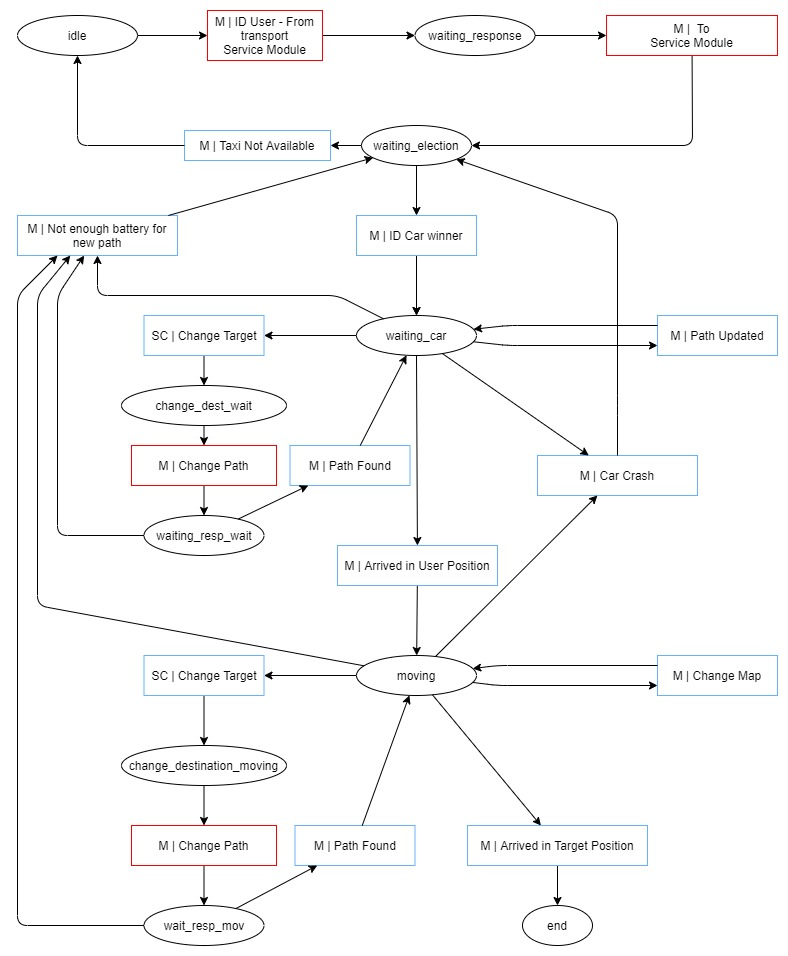
\includegraphics[width=15cm]{automa_utente.jpg}
	\caption{Rappresentazione degli stati possibili dell'entità utente.}
	\label{fig:automa_utente}
\end{figure}

L'immagine \ref{fig:automa_macchina} rappresenta l'automa degli stati dell'entità macchina.


\begin{figure}[htbp]
	\centering
	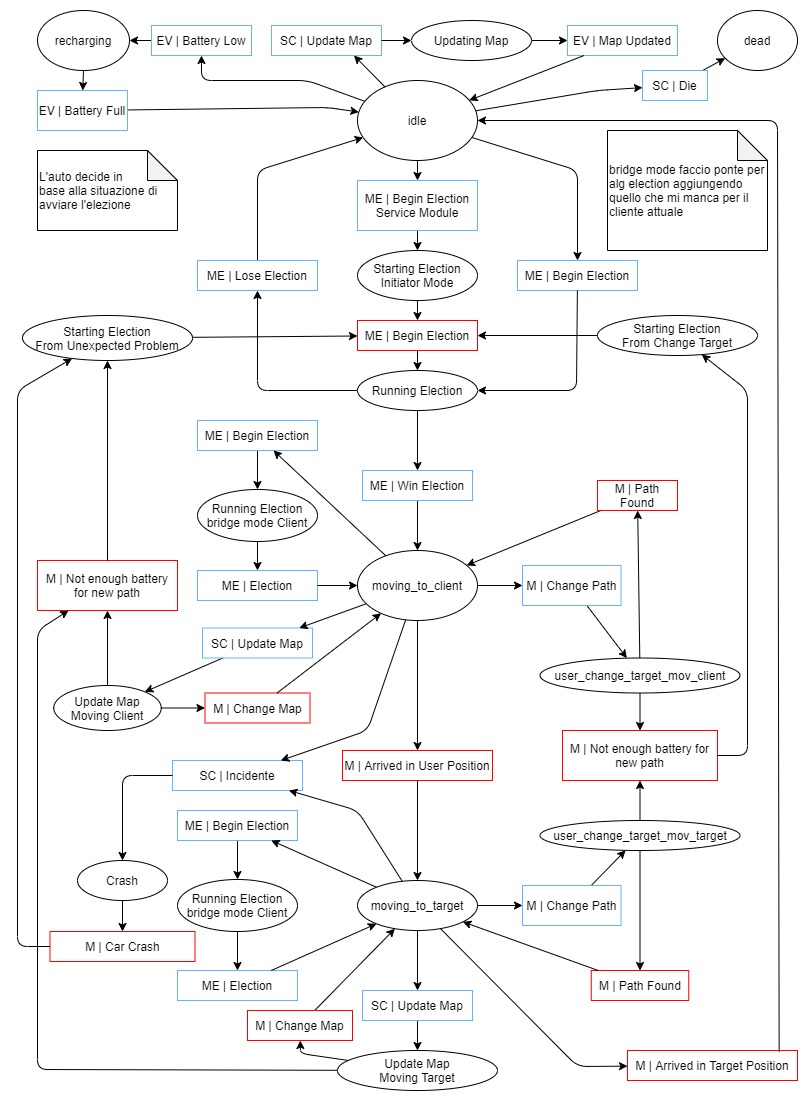
\includegraphics[width=15cm]{automa_macchina.jpg}
	\caption{Rappresentazione degli stati possibili dell'entità macchina.}
	\label{fig:automa_macchina}
\end{figure}

\newpage

\section{Protocolli e algoritmi}
In questa sezione vengono discusse le comunicazioni tra le diverse componenti e gli algoritmi utilizzati all'interno del sistema.

\subsection{Funzioni di costo delle macchine} \label{funzioni_di_costo_macchine}
Per la scelta della macchina più adatta, vengono considerati i seguenti parametri.

\begin{itemize}
	\item Crdt = Carica Rimanente Dopo Trasporto dell'utente.
	\item Cc = Costo Cliente, esprime dopo quanto tempo la macchina raggiungerebbe il cliente.
	\item Cr = Carica Rimanente espressa in unità di misura della distanza percorribile.
	\item Prc = Percorso Rimanente Cliente espresso in unità di misura della distanza assumendo che il taxi sia occupato.
	\item Pvcn = Percorso Verso Cliente Nuovo a partire dalla posizione dopo lo scorso cliente espresso in unità di misura della distanza.
	\item Pvdc = Percorso Verso Destinazione Cliente a partire dalla posizione attuale del cliente espresso in unità di misura della distanza.
	\item Pvcr = Percorso Verso Colonnina Ricarica per permettere alla macchina di ricaricarsi dopo il trasporto se necessario.
\end{itemize}

\begin{equation} \label{funzione_costo_raggiungimento_cliente}
Cc = Prc + Pvcn
\end{equation}

\begin{equation} \label{carica_rimanente_trasporto}
Crdt = Cr - (Cc + Pvdc + Pvcr)
\end{equation}

La scelta della macchina, verrà effettuata minimizzando il tempo del cliente \ref{funzione_costo_raggiungimento_cliente} e, in caso di parità, massimizzando la carica rimanente dopo il trasporto \ref{carica_rimanente_trasporto}. Nel caso in cui non sia univoco il vincitore, la selezione diventa casuale tra i contendenti.

\subsection{Pacchetti scambiati per l'elezione}\label{descrizione_pacchetto}
Vengono utilizzati tre tipi di pacchetti per l'algoritmo di elezione:
\begin{itemize}
	\item Inizio algoritmo elezione
	\item Risultati dei calcoli
	\item Notifica Vincitore
\end{itemize}

\subsubsection{Inizio algoritmo}
Lo scopo di questo pacchetto è di notificare ai nodi raggiungibili dal nodo corrente l'inizio dell'elezione. Esso è formato in questo modo:

\begin{lstlisting}
[ID_self, begin_election, TTL]
\end{lstlisting}

\begin{itemize}
	\item ID\_self: il riferimento a sé stesso per permettere l'impostazione del genitore agli altri nodi raggiunti.
	\item TTL: Per evitare di dover visitare tutto il grafo delle comunicazioni tra le macchine, si è scelto di impostare un TTL al pacchetto affiché dopo un certo numero fisso di salti ci si fermi. Questo porta al fatto che non è garantito che la soluzione trovata sia quella ottimale, tuttavia ciò permette un compromesso tra una buona soluzione e una limitazione della possibile congestione dei messaggi. Inoltre permette una riduzione dei possbili conflitti tra diverse leader election.
\end{itemize}

Il sistema si aspetta che alla ricezione di questo messaggio, il nodo risponda con una notifica di acknowledgment, in tal modo il nodo inviante è sicuro che esso sia stato ricevuto.

\subsubsection{Risultato dei calcoli} \label{pacchetto_calcolato}
Questo pacchetto contiene i dati calcolati dai nodi raggiunti dal pacchetto "inizio algoritmo" assieme a quelli del nodo corrente. Esso verrà poi inviato al genitore e sempre tramite esso è possibile creare la tabella di routing dei nodi coinvolti nell'elezione. Tuttavia per la comunicazione del vincitore, non verrà utilizzata la suddetta tabella poiché è più efficiente effettuare un multicast.

\begin{lstlisting} 
[{ID_1, Cc_1, Crdt_1}, ..., {ID_N, Cc_N, Crdt_N}]
\end{lstlisting}

Esso contiene, in ordine, per ogni nodo i: 
\begin{itemize}
	\item ID\_i: riferimento al veicolo i.
	\item Cc\_i, Crdt\_i: i costi della macchina i come descritto nella funzione di costo \ref{funzioni_di_costo_macchine}
\end{itemize}

\subsubsection{Notifica Vincitore}\label{pacchetto_vincitore}
Scopo del pacchetto è di notificare il vincitore dell'elezione e rilasciare i nodi coinvolti in essa. Questo pacchetto è formato nel seguente modo:

\begin{lstlisting}
[ID_WINNER, winner]
\end{lstlisting}

Il nodo iniziatore lo crea e lo invia in multicast a tutti i nodi coinvolti nell'elezione.

Successiva

\subsection{Creazione dello Spanning Tree}

Per l'elezione è necessaria la creazione di uno Spanning Tree dei nodi partecipanti ad essa per le comunicazioni. L'Echo algoritm che viene utilizzato ne permette la creazione man mano che i nodi ricevono i messaggi di inizio elezione.

Ogni nodo che partecipa riceve dal genitore padre la notifica di inizio elezione e in tal modo viene creata una relazione padre-figlio tramite la quale possono comunicare. Se un nodo riceve lo stesso tipo di notifica ma possiede già un padre, risponde al mittente di non poter partecipare e non inoltra ai propri vicini la notifica.

La radice dello spanning tree è il nodo iniziatore.

\subsection{Algoritmo di Elezione}

Come già accennato nell'introduzione al punto \ref{intro_algo}, l'algoritmo di elezione scelto è di tipo Wave e ne soddisfa le notorie proprietà. In particolare, si è optato per un Echo algoritm poichè il grafo su cui deve essere applicato è indiretto ed è possibile che siano presenti dei cicli.
L'algoritmo segue i seguenti passi:

\begin{enumerate}
	\item La macchina iniziatrice, la quale viene scelta perché la più vicina al cliente oppure in seguito a degli eventi di aggiornamento della mappa o incidente, inizia la wave creando un pacchetto da inviare ai propri vicini formato come già descritto al punto \ref{descrizione_pacchetto}, poi calcola i propri costi come descritto nella parte \ref{funzioni_di_costo_macchine}, ed aspetta i dati dei nodi che hanno risposto in modo positivo con l'acknowledgment al pacchetto di inizio elezione.
	\item Ogni nodo che riceve il pacchetto di inizio elezione, se non sta già partecipando a un'altra elezione, si sposta nello stato relativo al calcolo del leader. In ogni caso, risponde al nodo inviante se partecipa oppure no all'elezione. In caso negativo, non inoltra il pacchetto di inizio elezione ricevuto ai suoi vicini. In caso positivo, invece, se il TTL è superiore a 0, ne riduce il valore di un'unità e lo inoltra ai propri vicini. Successivamente, come per il nodo padre, si mette in attesa degli ack dei vicini.
	\item Il nodo che riceve il pacchetto di starting election con TTL pari a zero, dopo avere inviato l'ack al genitore, non inoltra ulteriormente l'inizio dell'elezione ai vicini.
	\item Ogni nodo, dopo aver ricevuto l'ack da parte dei figli alla partecipazione dell'elezione, calcola i propri costi e si mette in attesa che i propri figli, se presenti, gli mandino i costi calcolati. Alla ricezione di tutti i costi dei figli esso crea un pacchetto unico concatenando i costi ricevuti al proprio. Successivamente inoltre il pacchetto risultate al padre. Per la struttura di esso si faccia riferimenti a \ref{pacchetto_calcolato}.
	\item Dopo aver inviato al padre i dati relativi ai costi, ogni nodo si mette in attesa di conoscere chi è il leader.
	\item Quando il nodo iniziatore riceve tutti i dati calcola il leader in base alle proprietà descritte nella parte \ref{funzioni_di_costo_macchine}. 
	\item Infine l'iniziatore invia il messaggio contentente il leader in multicasting a tutti i partecipanti all'elezione. Si faccia rifermento alla parte \ref{pacchetto_vincitore} per la descrizione del pacchetto.
	\item Tutti i nodi ricevono la notifica del leader e in base al risultato compiono le azioni più opportune. In ogni caso escono dallo stato di elezione eliminando tutte le informazioni calcolate.
	\item Il nodo vincitore comunica al moudlo di ricezione del cliente, tramite le celle di comunicazione descritte nell'introduzione al punto \ref{problematiche_distribuite}, di essere pronto a servirlo e se egli è in coda oppure no.
\end{enumerate}

Un esempio dei pacchetti scambiati durate l'algoritmo è presente all'immagine \ref{fig:messaggi_macchina_elezione}. La parte in basso a sinistra mostra lo spanning tree creato.

\begin{figure}[htbp]
	\centering
	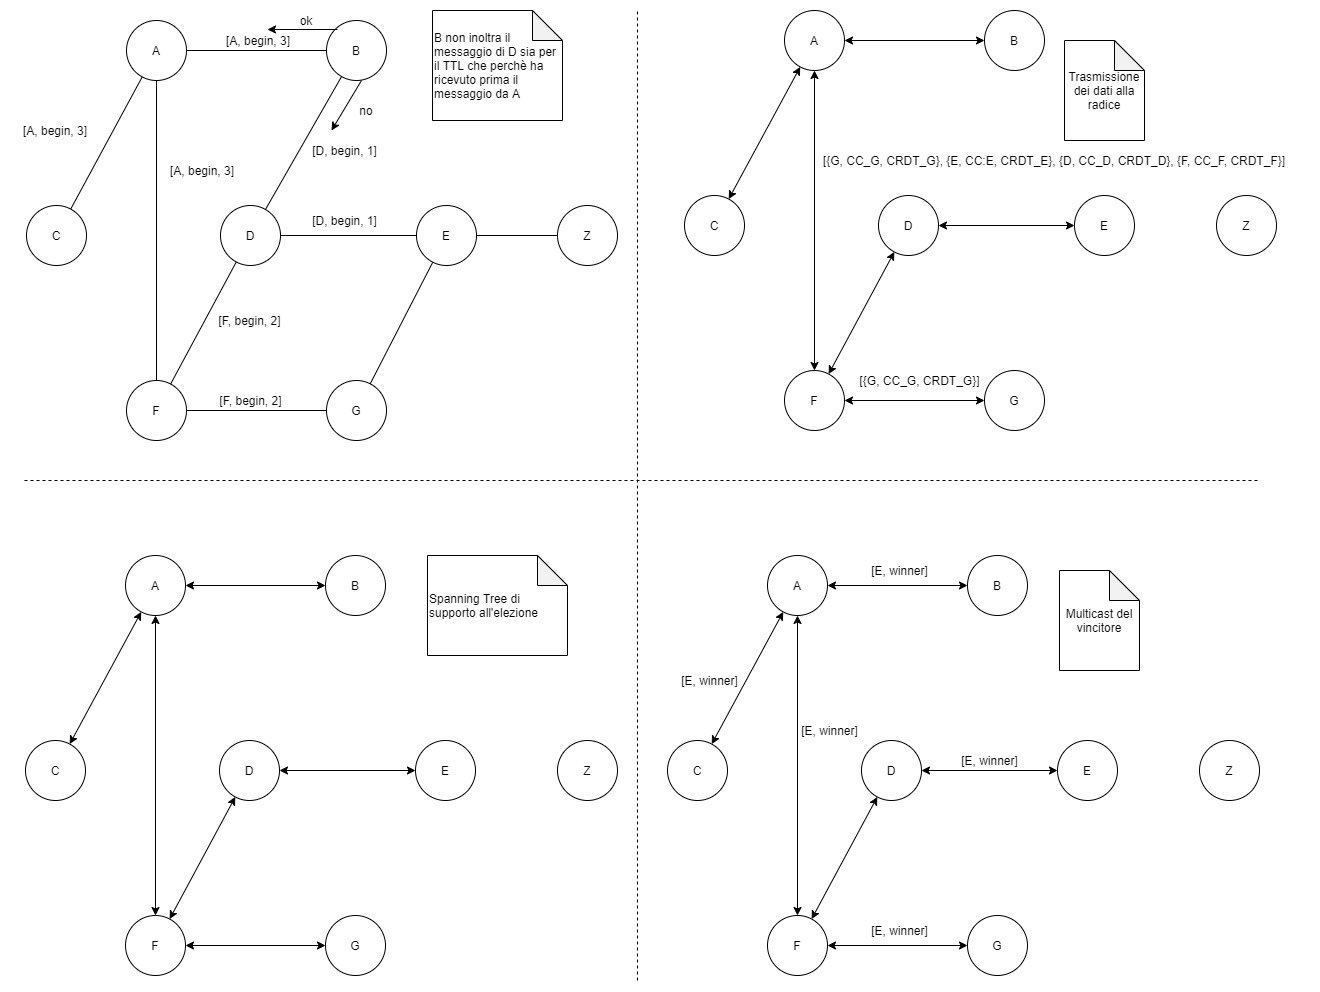
\includegraphics[width=15cm]{messaggi_macchina_elezione.jpg}
	\caption{Rappresentazione dei messaggi scambiati durante l'elezione.}
	\label{fig:messaggi_macchina_elezione}
\end{figure}

\newpage

\subsection{Possibili errori durante l'elezione}

I problemi durante l'esecuzione dell'algoritmo nel sistema sono i seguenti:
\begin{itemize}
	\item Aggiornamento della mappa.
\end{itemize}

I problemi possibili ma assenti per via dell'implementazione del sistema sono i seguenti:
\begin{itemize}
	\item Rimozione di una macchina
	\item Perdita di pacchetti
\end{itemize}

\subsubsection{Aggiornamento della mappa}
Viene discussa nella sezione Aggiornamento Mappa \ref{aggiornamento_mappa}.

\subsubsection{Rimozione di una macchina}
Sebbene il sistema venga costruito in modo che un nodo possa essere rimosso solamente se si trova nello stato "idle", è bene gestire i casi in cui l'eliminazione avvenga in ogni possibile stato, compresa l'elezione. Per risolvere il problema di attesa della risposta da un nodo ormai rimosso, ogni nodo invia dei messaggi di tipo "hello" per controllare lo stato del nodo collegato. In tal modo se non ricevono risposta entro un tempo ragionevole lo considerano rimosso e continuano l'algoritmo di elezione.

\subsubsection{Perdita di pacchetti}
Nel caso in cui vengano persi dei pacchetti durante qualsiasi fase dell'elezione, è possibile accorgersene poichè non ritornano i messaggi di ack. Una possibile soluzione per questo problema è l'utilizzo del protocollo TCP.

\subsection{Aggiornamento della mappa}\label{aggiornamento_mappa}

Questa casistica comporta che i percorsi calcolati, nel caso utilizzino degli archi deprecati, non siano più validi. 

L'aggiornamento può avvenire in diversi momenti e stati della macchina. 

\begin{itemize}
	\item Macchina in stato IDLE: Semplice aggiornamento, non comporta alcun problema.
	\item Macchina in stato Running Election: al termine dell'elezione effettua l'aggiornamento. Se risulta vincitrice ed è necessario, ricalcola il percorso.
	\item Macchina in stato Moving to Client o Moving to Target con un solo cliente: il veicolo effettua l'aggiornamento della mappa e, se necessario, ricarcola il percorso. Se è in grado di soddisfare l'utente, lo notifica del ritardo e torna nello stato precedente. Altrimenti notifica l'utente e inizia una leader election per l'utente.
	\item Macchina in stato Moving to Client o Moving to Target con più clienti in coda: Effettua l'aggiornamento e calcola il massimo percorso che riesce a soddifare con la carica rimanente. In tal modo, nel caso in cui alcuni clienti non possano venir soddifatti li notifica con un messaggio di avviare autonomamente una nuova richiesta al sistema e li rimuove dalla coda. In questo caso non parte alcuna leader election. Nel caso peggiore in cui non riesca a soddisfare nemmeno il cliente corrente l'approccio è come al punto precedente.
	\item Macchina in stato Running Election Bridge Mode: come detto precedentemente, esegue comunque il calcolo del leader e poi si comporta in base al numero di utenti in coda.
\end{itemize}

\subsection{Diagrammi di sequenza dei messaggi}
All'appendice \ref{messaggi_scambiati_appendix}, sono presenti i diagrammi di sequenza dei messaggi che vengono scambiati tra i diversi moduli per permettere le funzionalità del sistema.

\begin{itemize}
	\item Richiesta da parte dell'utente del servizio di trasporto \ref{fig:messaggi_utente_chiede_macchina}.
	\item Movimento del taxi alla posizione dell'utente e successivo trasporto \ref{fig:messaggi_utente_trasporto}.
	\item Richiesta di cambiamento di destinazione da parte dell'utente mentre il taxi è in viaggio verso l'utente \ref{fig:messaggi_utente_cambio_direzione_waiting}.
	\item Richiesta di cambiamento di destinazione da parte dell'utente mentre il taxi lo sta trasportando \ref{fig:messaggi_utente_cambio_direzione_moving}.
	\item Partecipazione all'elezione di una macchina non iniziatrice \ref{fig:messaggi_macchina_partecipazione_elezione}. Poiché è possibile che la macchina si trovi in diversi stati mentre viene avviato l'algoritmo di elezione, sono stati rappresentati tre possibili scenari.
	\item Incidente di una macchina con conseguente notifica all'utente e ricerca di un taxi alternativo \ref{fig:messaggi_macchina_crash}.
	\item Ricarica della macchina, rimozione della macchina dal sistema e aggiornamento della mappa  \ref{fig:messaggi_macchina_batteria_morte_mappaIdle}. In queste operazioni si considera che la macchina sia nello stato 'idle'.
	\item Aggiornamento della mappa della città mentre il taxi si sta muovendo verso il cliente \ref{fig:messaggi_macchina_aggiornamento_mappa_to_client}.
	\item Aggiornamento della mappa della città mentre il taxi sta trasportando il cliente a destinazione \ref{fig:messaggi_macchina_aggiornamento_mappa_to_target}.
	\item Aggiornamento della mappa della città mentre il taxi è occupato con un utente e ne ha altri nella coda \ref{fig:messaggi_macchina_aggiornamento_mappa_clienti}.
\end{itemize}


\section{Architettura fisica e Distribuzione} \label{arch_fisica}
Per l'implementazione fisica del progetto, è necessario che ogni automobile elettrica sia dotata di una scheda Wi-Fi per la comunicazione con i veicoli vicini. Il cliente per poter comunicare con il sistema necessita di utilizzare un'applicazione dedicata per le prenotazioni. Si suppone esista già la mappa della città nel formato adatto, ogni automobile deve possederne una copia nel disco locale. Un altro requisito hardware è che le macchine dispongano di sufficiente potenza di calcolo per effettuare velocemente il calcolo dei percorsi.

I moduli descritti nella sezione \ref{modules} sono associati ai componenti fisici in questo modo:
I moduli per le operazioni sui grafi, la scheda wireless, operazioni mappa città, gestione macchine, elezione del leader sono legati ai taxi e il modulo entità macchina ne rappresenta una sua astrazione.

Il modulo per l'interfaccia cliente-servizio è legato all'utente, esso infatti deve conoscere soltanto questo modulo per utilizzare il servizio, il modulo utente ne rappresenta una sua astrazione.

il "modulo per l'invio dei messaggi" è utilizzato da tutti i componenti, in quanto l'invio di un qualsiasi messaggio viene analizzato dai metodi di questo modulo.

I moduli per le operazioni sui grafi, operazioni mappa città, gestione macchine, comunicazione ambiente-entità, creazione entità vengono usati dall'ambiente, il quale però, si ricorda, non ha nessuna rappresentazione nei componenti fisici del sistema.

una descrizione delle dipendenze fra i moduli verrà rappresentata da un grafo...

\begin{itemize} 
	
	\item Modulo algoritmi grafi: fornisce gli algoritmi che è possibile utilizzare sui grafi. Per esempio include Dijkstra, BFS, DFS, aggiungi nodo, aggiungi arco, ... 
	
	\item Modulo per l'algoritmo di elezione del leader: implementa la funzionalità della scelta della macchina da assegnare all'utente.
	
	\item Modulo per l'invio di messaggi: controlla che il messaggio sia ben formato.
	
	\item Modulo interfaccia cliente-servizio: fornisce le possibili operazioni che un cliente può richiedere al sistema.
	
	\item Modulo scheda wireless: simula la scheda di rete che fornisce i vicini dell'entità che ne invoca i metodi.
	
	\item Modulo mappa città: fornisce i metodi di lettura e modifica della mappa della città.
	
	\item Modulo gestione macchine: fornisce i metodi per ricaricare le batterie delle macchine, ne gestiscono gli incidenti e le riparazioni.
	
	\item Modulo creazione entità: fornisce le primitive per creare nuove macchine e nuovi utenti.
	
	\item Modulo comunicazione Ambiente-Entità: il processo Ambiente può utilizzare i metodi in questo modulo per simulare il mondo reale.
	
	\item Modulo Entità Macchina: rappresenta l'astrazione dell'entità veicolo.
	
	\item Modulo Entità Utente: rappresenta l'astrazione dell'entità utente.
	
	\item Modulo Entità Ambiente : rappresenta l'astrazione dell'entità ambiente.
	
	L'associazione fra i componenti fisici del sistema con i suddetti moduli e le varie dipendenze fra questi sono riportate nella sezione \ref{arch_fisica}.
\end{itemize}

\section{Piano di Sviluppo}
% Since it is diffcult to predict just how hard implementing a new system will be, you should formulate as a set of "tiers", where the basic tier is something youre sure you can complete, and the additional tiers add more features, at both the application and the system level.

Sono stati individuati due insiemi di funzionalità che è necessario supportare.
\subsection{Funzionalità Base}

\begin{enumerate}
	\item Comunicazione peer to peer per la leader election.
	\item Richiesta dell'utente di trasporto.
	\item Gestione della ricarica delle macchine.
	\item Cambio di direzione di utente singolo.
	\item Gestione degli incidenti sia delle macchine che delle strade rotte.
\end{enumerate}

\subsection{Funzionalità Aggiuntive}

\begin{itemize}
	\item Perdita delle connessioni mentre si elegge il leader.
	\item Partecipazione della macchina già impegnata alla leader election.
	\item Possibilità di rimuovere la prenotazione
	\item Possibilità di cambiare destinazione anche se ci sono altri utenti nella coda della macchina candidata. Questa funzionalità vale per tutti gli utenti in coda, tuttavia è limitata dalla nuova destinazione che deve costare meno rispetto alla precedente.
	\item Car sharing fino a tre persone.
\end{itemize}

\subsection{Ordine di sviluppo}
Lo sviluppo dell'applicazione verrà suddiviso in diverse versioni via via estese con le nuove funzionalità. In particolare si seguirà questo ordine:

\begin{enumerate}
	\item Ogni macchina potrà parlare con tutte le altre macchine; l'utente invia la richiesta di trasporto alla macchina più vicina a lui; se un veicolo è impegnato con un cliente non partecipa alla selezione del leader per il trasporto ma fa da ponte per i vicini; la comunicazione tra i veicoli è diretta, quindi ogni taxi può parlare con chiunque.
	\item Vengono aggiunte le colonnine di ricarica, alle quali le macchine devono far rifornimento se stanno esaurendo le batterie; le macchine possono guastarsi; l'utente può decidere di cambiare destinazione.
	\item Rottura delle strade ma senza disconnessione del grafo stradale.
	\item Le macchine possono comunicare solo con quelle vicine.
	\item La macchina partecipa all'elezione anche se al momento è già impegnata, tuttavia si considera disponibile solo dopo aver compiuto il tragitto già attivo.
	\item Le connessioni tra le macchine possono perdere andare perse mentre si elegge il leader.
	\item Rimuovere prenotazione.
	\item Cambio direzione anche se in lista.
	\item Implementazione del car-sharing fino a 3 clienti.
\end{enumerate}